%---------------------------------------------------------------
\chapter{\babLima}
%---------------------------------------------------------------

%---------------------------------------------------------------
\section{Hasil Pengolahan Data Jarak}
%---------------------------------------------------------------
\subsection{Data Jarak 3 Meter}

\begin{figure}
    \centering
    \begin{subfigure}[b]{0.45\textwidth}
        \centering
        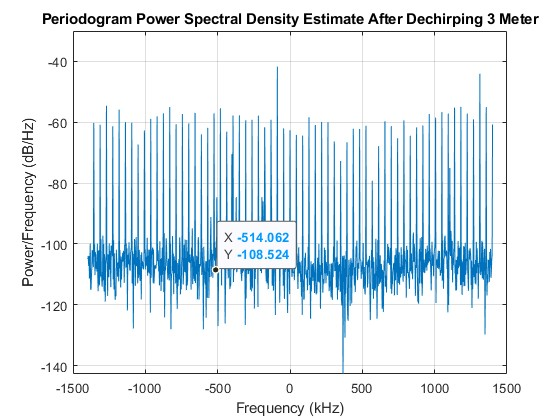
\includegraphics[scale=0.35]{pics/bab5/Range/1_3.jpg}
        \caption{Nilai \textit{beat frequency} 3 meter pengulangan 1}
        \label{fig:pengambilan3_1}
    \end{subfigure}
    \hfill
    \begin{subfigure}[b]{0.45\textwidth}
        \centering
        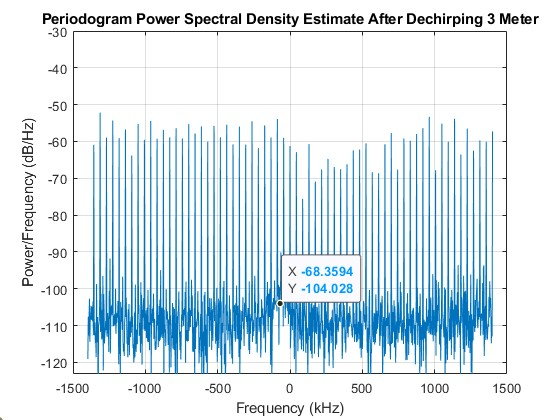
\includegraphics[scale=0.35]{pics/bab5/Range/2_3.jpg}
        \caption{Nilai \textit{beat frequency} 3 meter pengulangan 2}
        \label{fig:pengambilan3_2}
    \end{subfigure}
    \vskip\baselineskip
    \begin{subfigure}[b]{0.6\textwidth}
        \centering
        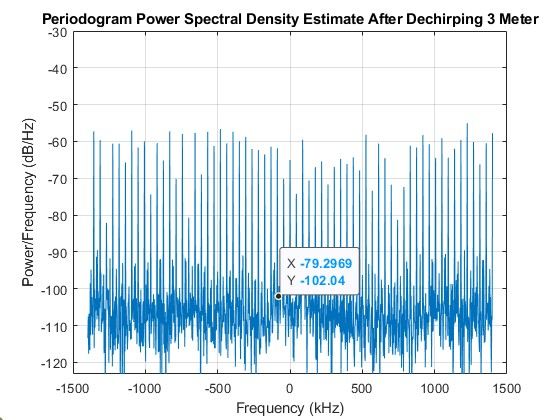
\includegraphics[scale=0.35]{pics/bab5/Range/3_3.jpg}
        \caption{Nilai \textit{beat frequency} 3 meter pengulangan 3}
        \label{fig:pengambilan3_3}
    \end{subfigure}
    \caption{Hasil \textit{beat frequency} dari jarak 3 meter}
    \label{fig:pengambilan3}
\end{figure}

Pada gambar~\ref{fig:pengambilan3} telah dilampirkan tiga hasil percobaan pengambilan data jarak objek setelah diolah dengan matlab untuk mendapatkan nilai \textit{beat frequency} dari objek. Pada gambar~\ref{fig:pengambilan3_1} yang menunjukkan pengambilan data pengulangan pertama didapatkan hasil nilai \textit{beat frequency} pada frekuensi -601.562 Khz, pada gambar~\ref{fig:pengambilan3_2} yang menunjukkan pengambilan data pengulangan kedua didapatkan nilai -546.875 kHz, dan pada pengambilan data pengulangan ketiga, nilai \textit{beat frequency} adalah -1941.41 kHz seperti pada gambar~\ref{fig:pengambilan3_3}.

\subsection{Data Jarak 6 Meter}

\begin{figure}
    \centering
    \begin{subfigure}[b]{0.45\textwidth}
        \centering
		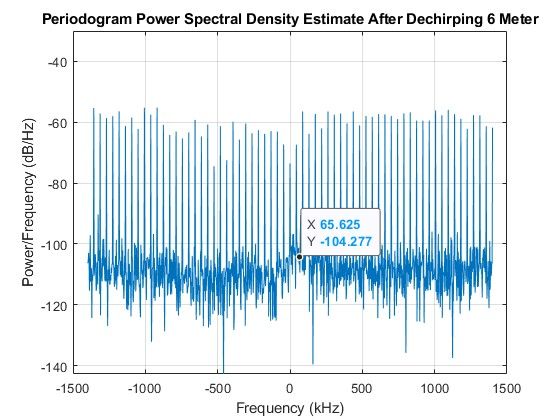
\includegraphics[scale=0.35]{pics/bab5/Range/1_6.jpg}
		\caption{Nilai \textit{beat frequency} 6 meter pengulangan 1}
		\label{fig:pengambilan6_1}
    \end{subfigure}
    \hfill
    \begin{subfigure}[b]{0.45\textwidth}
        \centering
		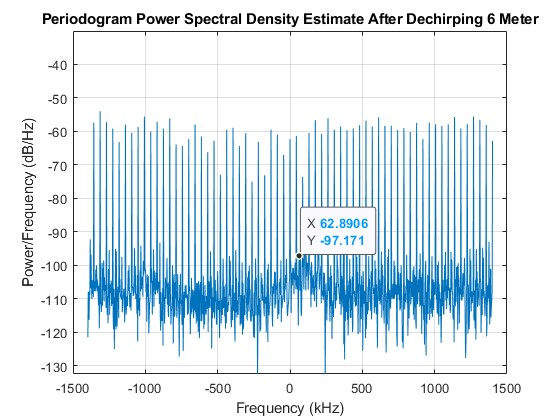
\includegraphics[scale=0.35]{pics/bab5/Range/2_6.jpg}
		\caption{Nilai \textit{beat frequency} 6 meter pengulangan 2}
		\label{fig:pengambilan6_2}
    \end{subfigure}
    \vskip\baselineskip
    \begin{subfigure}[b]{0.6\textwidth}
        \centering
		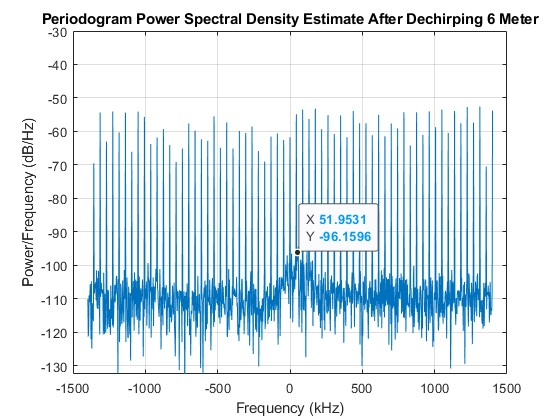
\includegraphics[scale=0.35]{pics/bab5/Range/3_6.jpg}
		\caption{Nilai \textit{beat frequency} 6 meter pengulangan 3}
		\label{fig:pengambilan6_3}
    \end{subfigure}
    \caption{Hasil \textit{beat frequency} dari jarak 6 meter}
    \label{fig:pengambilan3}
\end{figure}

Pada gambar~\ref{fig:pengambilan6} telah dilampirkan tiga hasil percobaan pengambilan data jarak objek setelah diolah dengan matlab untuk mendapatkan nilai \textit{beat frequency} dari objek. Pada gambar~\ref{fig:pengambilan6_1} yang menunjukkan pengambilan data pengulangan pertama didapatkan hasil nilai \textit{beat frequency} pada frekuensi 464.844 Khz, pada gambar~\ref{fig:pengambilan6_2} yang menunjukkan pengambilan data pengulangan kedua didapatkan nilai 628.906 kHz, dan pada pengambilan data pengulangan ketiga, nilai \textit{beat frequency} adalah 519.531 kHz seperti pada gambar~\ref{fig:pengambilan6_3}.

\subsection{Data Jarak 9 Meter}

\begin{figure}
    \centering
    \begin{subfigure}[b]{0.45\textwidth}
        \centering
		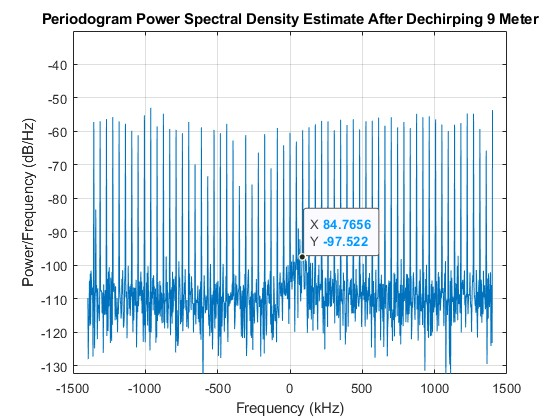
\includegraphics[scale=0.3]{pics/bab5/Range/1_9.jpg}
		\caption{Nilai \textit{beat frequency} 9 meter pengulangan 1}
		\label{fig:pengambilan9_1}
    \end{subfigure}
    \hfill
    \begin{subfigure}[b]{0.45\textwidth}
        \centering
		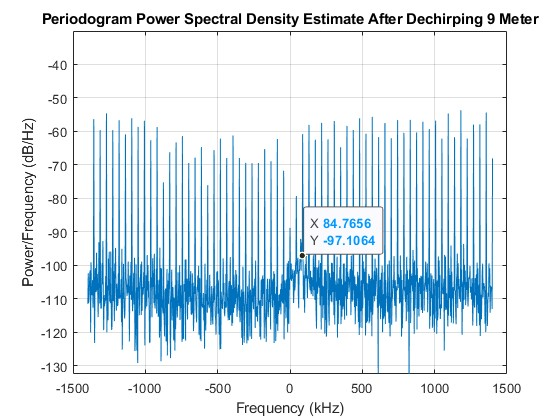
\includegraphics[scale=0.35]{pics/bab5/Range/2_9.jpg}
		\caption{Nilai \textit{beat frequency} 9 meter pengulangan 2}
		\label{fig:pengambilan9_2}
    \end{subfigure}
    \vskip\baselineskip
    \begin{subfigure}[b]{0.6\textwidth}
        \centering
		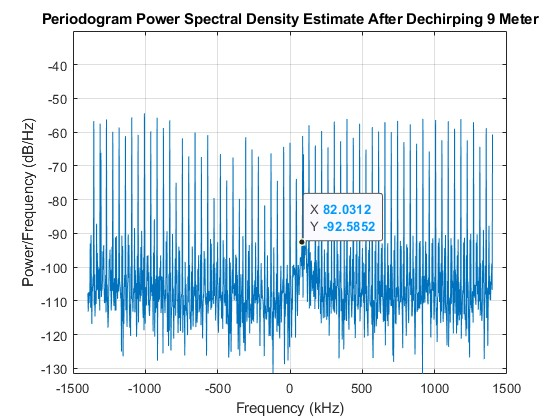
\includegraphics[scale=0.35]{pics/bab5/Range/3_9.jpg}
		\caption{Nilai \textit{beat frequency} 9 meter pengulangan 3}
		\label{fig:pengambilan9_3}
    \end{subfigure}
    \caption{Hasil \textit{beat frequency} dari jarak 9 meter}
    \label{fig:pengambilan9}
\end{figure}

Pada gambar~\ref{fig:pengambilan9} telah dilampirkan tiga hasil percobaan pengambilan data jarak objek setelah diolah dengan matlab untuk mendapatkan nilai \textit{beat frequency} dari objek. Pada gambar~\ref{fig:pengambilan9_1} yang menunjukkan pengambilan data pengulangan pertama didapatkan hasil nilai \textit{beat frequency} pada frekuensi 847.666 Khz, pada gambar~\ref{fig:pengambilan9_2} yang menunjukkan pengambilan data pengulangan kedua didapatkan nilai 847.656 kHz, dan pada pengambilan data pengulangan ketiga, nilai \textit{beat frequency} adalah 820.312 kHz seperti pada gambar~\ref{fig:pengambilan9_3}.

%---------------------------------------------------------------
\section{Hasil Pengolahan Data Kecepatan}
%---------------------------------------------------------------

\subsection{Data Kecepatan 5 km/h}

\begin{figure}
	\centering
	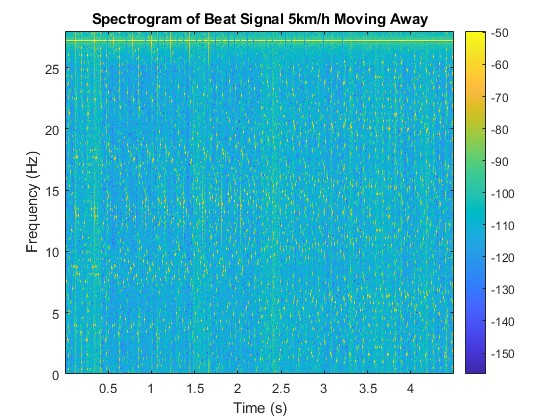
\includegraphics[scale=0.6]{pics/bab5/Velocity/1_5MA.jpg}
	\caption{Perubahan Jarak dari objek Menjauhi Radar dengan kecepatan 5 km/h pengulangan 1}
	\label{fig:pengambilan1_5MA}
\end{figure}

Pengambilan 1 5 MA

\begin{figure}
	\centering
	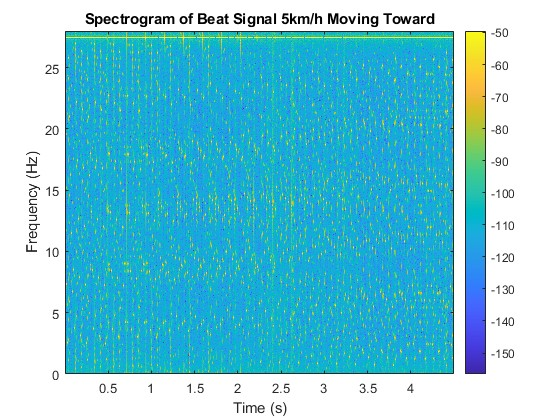
\includegraphics[scale=0.6]{pics/bab5/Velocity/1_5MT.jpg}
	\caption{Perubahan Jarak dari objek Mendekati Radar dengan kecepatan 5 km/h pengulangan 1}
	\label{fig:pengambilan1_5MT}
\end{figure}

Pengambilan 1 5 MT

\begin{figure}
	\centering
	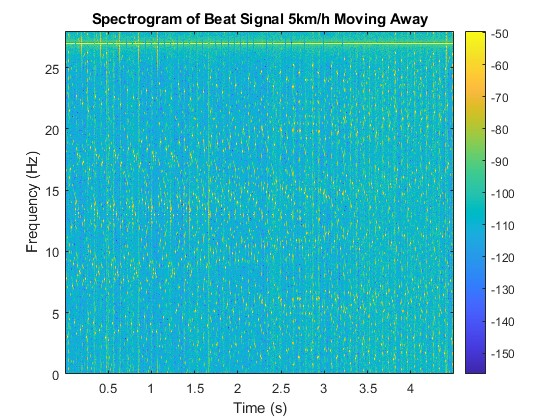
\includegraphics[scale=0.6]{pics/bab5/Velocity/2_5MA.jpg}
	\caption{Perubahan Jarak dari objek Menjauhi Radar dengan kecepatan 5 km/h pengulangan 2}
	\label{fig:pengambilan2_5MA}
\end{figure}

Pengambilan 2 5 MA

\begin{figure}
	\centering
	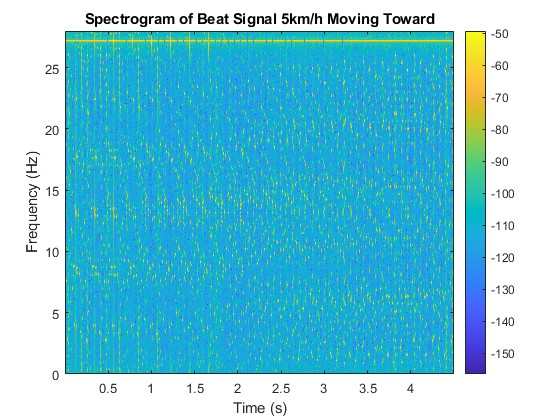
\includegraphics[scale=0.6]{pics/bab5/Velocity/2_5MT.jpg}
	\caption{Perubahan Jarak dari objek Mendekati Radar dengan kecepatan 5 km/h pengulangan 2}
	\label{fig:pengambilan2_5MT}
\end{figure}

Pengambilan 2 5 MT

\begin{figure}
	\centering
	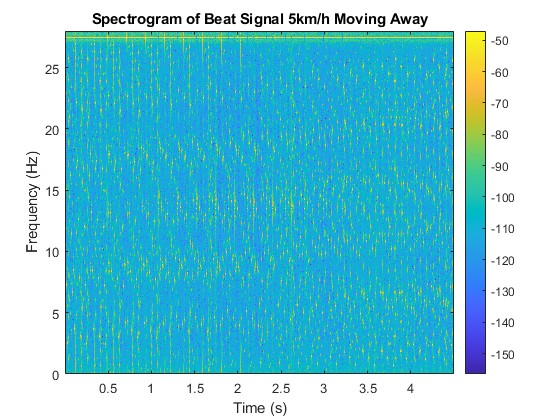
\includegraphics[scale=0.6]{pics/bab5/Velocity/3_5MA.jpg}
	\caption{Perubahan Jarak dari objek Menjauhi Radar dengan kecepatan 5 km/h pengulangan 3}
	\label{fig:pengambilan3_5MA}
\end{figure}

Pengambilan 3 5 MA

\begin{figure}
	\centering
	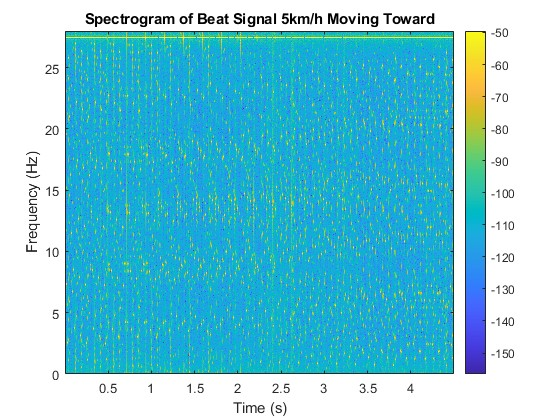
\includegraphics[scale=0.6]{pics/bab5/Velocity/1_5MT.jpg}
	\caption{Perubahan Jarak dari objek Mendekati Radar dengan kecepatan 5 km/h pengulangan 3}
	\label{fig:pengambilan3_5MT}
\end{figure}

Pengambilan 3 5 MT

\subsection{Data Kecepatan 10 km/h}

\begin{figure}
	\centering
	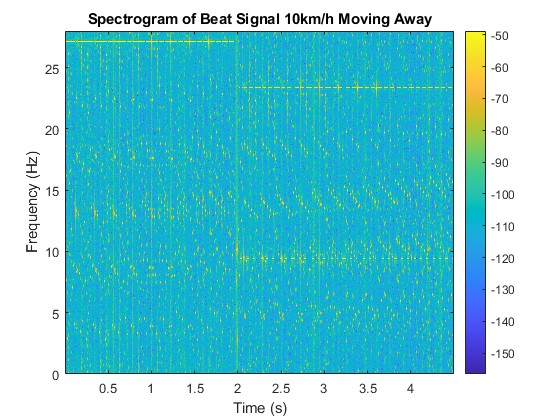
\includegraphics[scale=0.6]{pics/bab5/Velocity/1_10MA.jpg}
	\caption{Perubahan Jarak dari objek Menjauhi Radar dengan kecepatan 10 km/h pengulangan 1}
	\label{fig:pengambilan1_10MA}
\end{figure}

Pengambilan 1 10 MA

\begin{figure}
	\centering
	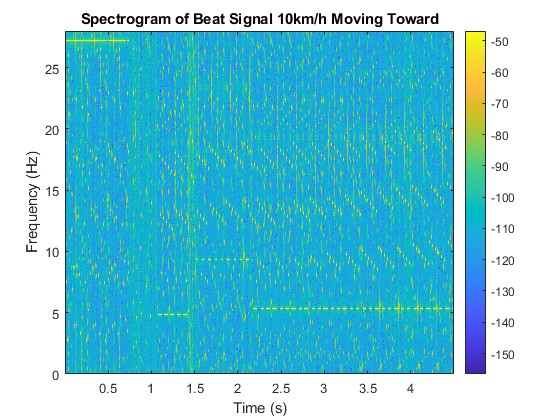
\includegraphics[scale=0.6]{pics/bab5/Velocity/1_10MT.jpg}
	\caption{Perubahan Jarak dari objek Mendekati Radar dengan kecepatan 10 km/h pengulangan 1}
	\label{fig:pengambilan1_10MT}
\end{figure}

Pengambilan 1 10 MT

\begin{figure}
	\centering
	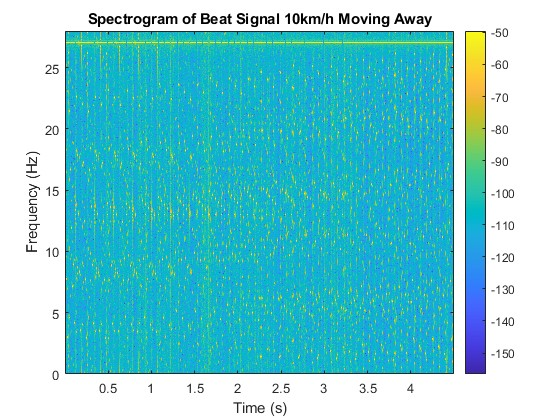
\includegraphics[scale=0.6]{pics/bab5/Velocity/2_10MA.jpg}
	\caption{Perubahan Jarak dari objek Menjauhi Radar dengan kecepatan 10 km/h pengulangan 2}
	\label{fig:pengambilan2_10MA}
\end{figure}

Pengambilan 2 10 MA

\begin{figure}
	\centering
	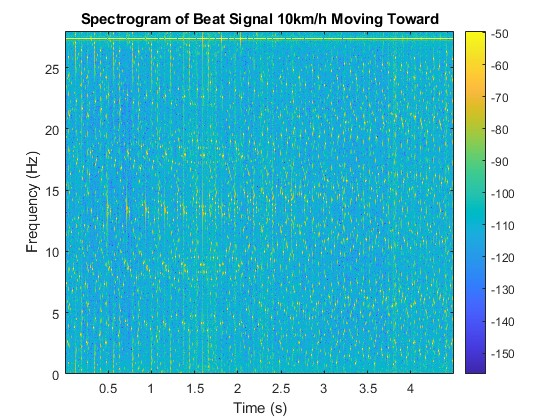
\includegraphics[scale=0.6]{pics/bab5/Velocity/2_10MT.jpg}
	\caption{Perubahan Jarak dari objek Mendekati Radar dengan kecepatan 10 km/h pengulangan 2}
	\label{fig:pengambilan2_10MT}
\end{figure}

Pengambilan 2 10 MT

\begin{figure}
	\centering
	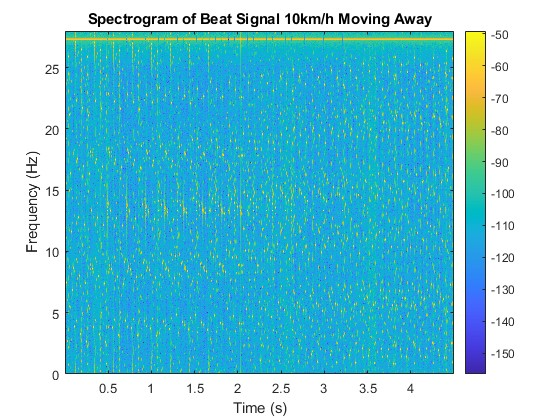
\includegraphics[scale=0.6]{pics/bab5/Velocity/3_10MA.jpg}
	\caption{Perubahan Jarak dari objek Menjauhi Radar dengan kecepatan 10 km/h pengulangan 3}
	\label{fig:pengambilan3_10MA}
\end{figure}

Pengambilan 3 10 MA

\begin{figure}
	\centering
	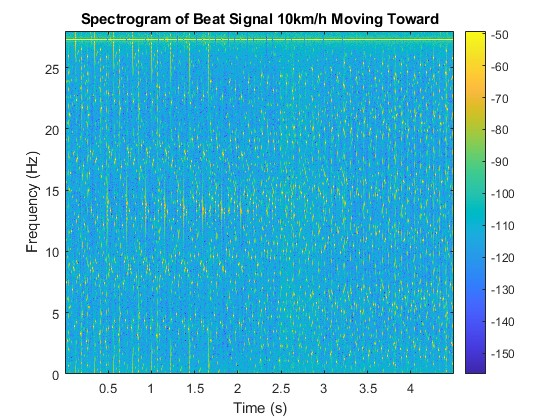
\includegraphics[scale=0.6]{pics/bab5/Velocity/3_10MT.jpg}
	\caption{Perubahan Jarak dari objek Mendekati Radar dengan kecepatan 10 km/h pengulangan 3}
	\label{fig:pengambilan3_10MT}
\end{figure}

Pengambilan 3 10 MT

\subsection{Data Kecepatan 15 km/h}

\begin{figure}
	\centering
	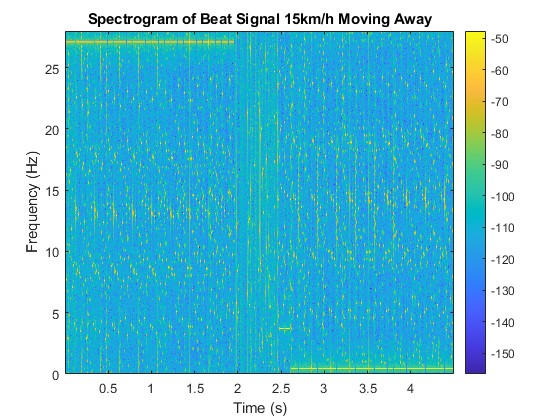
\includegraphics[scale=0.6]{pics/bab5/Velocity/1_15MA.jpg}
	\caption{Perubahan Jarak dari objek Menjauhi Radar dengan kecepatan 15 km/h pengulangan 1}
	\label{fig:pengambilan1_15MA}
\end{figure}

Pengambilan 1 15 MA

\begin{figure}
	\centering
	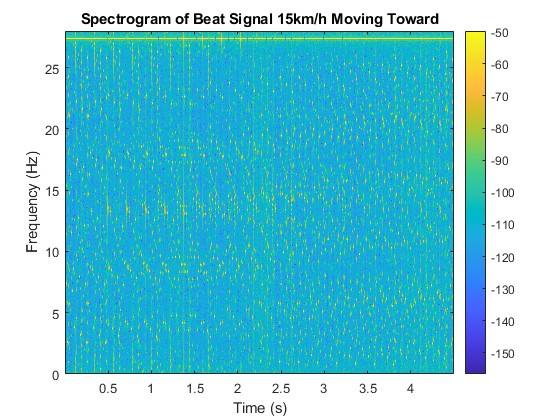
\includegraphics[scale=0.6]{pics/bab5/Velocity/1_15MT.jpg}
	\caption{Perubahan Jarak dari objek Mendekati Radar dengan kecepatan 15 km/h pengulangan 1}
	\label{fig:pengambilan1_15MT}
\end{figure}

Pengambilan 1 15 MT

\begin{figure}
	\centering
	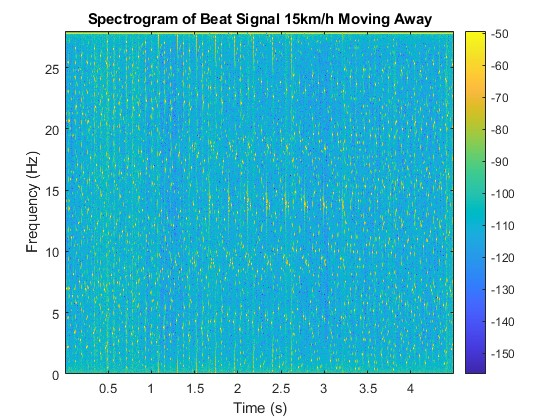
\includegraphics[scale=0.6]{pics/bab5/Velocity/2_15MA.jpg}
	\caption{Perubahan Jarak dari objek Menjauhi Radar dengan kecepatan 15 km/h pengulangan 2}
	\label{fig:pengambilan2_15MA}
\end{figure}

Pengambilan 2 15 MA

\begin{figure}
	\centering
	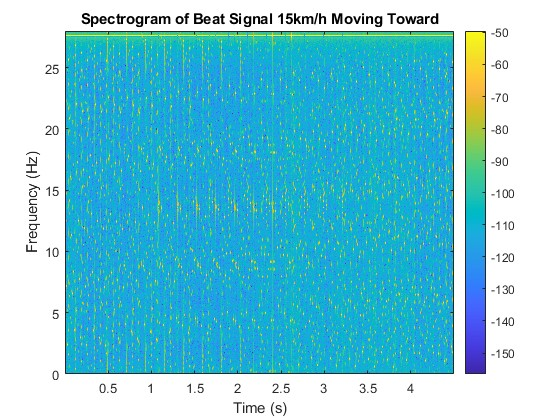
\includegraphics[scale=0.6]{pics/bab5/Velocity/2_15MT.jpg}
	\caption{Perubahan Jarak dari objek Mendekati Radar dengan kecepatan 15 km/h pengulangan 2}
	\label{fig:pengambilan2_15MT}
\end{figure}

Pengambilan 2 15 MT

\begin{figure}
	\centering
	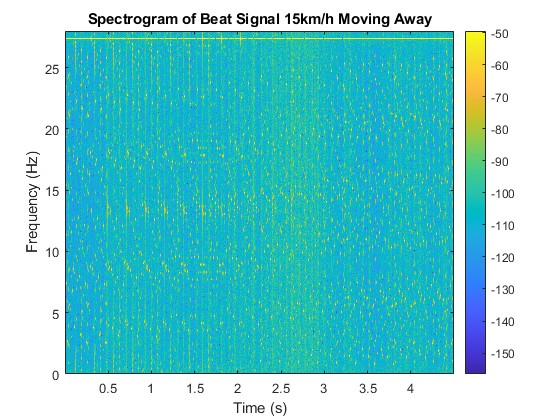
\includegraphics[scale=0.6]{pics/bab5/Velocity/3_15MA.jpg}
	\caption{Perubahan Jarak dari objek Menjauhi Radar dengan kecepatan 15 km/h pengulangan 3}
	\label{fig:pengambilan3_15MA}
\end{figure}

Pengambilan 3 15 MA

\begin{figure}
	\centering
	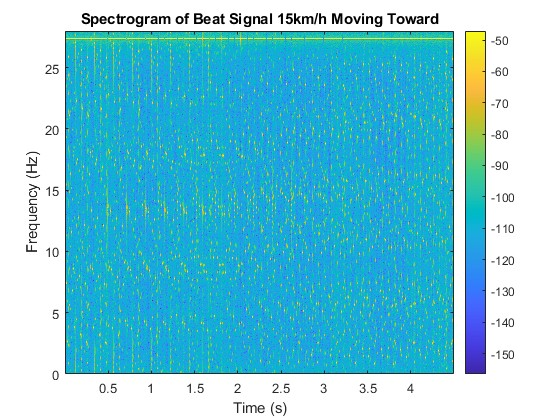
\includegraphics[scale=0.6]{pics/bab5/Velocity/3_15MT.jpg}
	\caption{Perubahan Jarak dari objek Mendekati Radar dengan kecepatan 15 km/h pengulangan 3}
	\label{fig:pengambilan3_15MT}
\end{figure}

Pengambilan 3 15 MT

\subsection{Data Kecepatan 20 km/h}

\begin{figure}
	\centering
	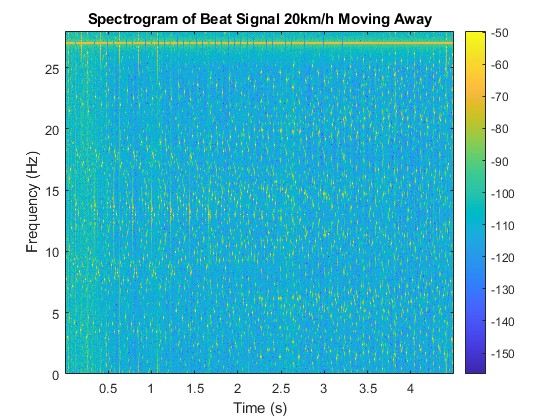
\includegraphics[scale=0.6]{pics/bab5/Velocity/1_20MA.jpg}
	\caption{Perubahan Jarak dari objek Menjauhi Radar dengan kecepatan 20 km/h pengulangan 1}
	\label{fig:pengambilan1_20MA}
\end{figure}

Pengambilan 1 20 MA

\begin{figure}
	\centering
	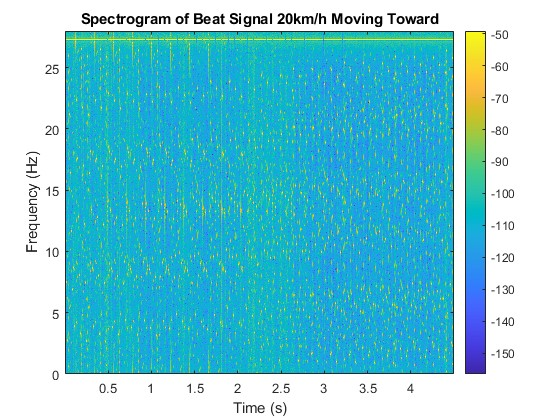
\includegraphics[scale=0.6]{pics/bab5/Velocity/1_20MT.jpg}
	\caption{Perubahan Jarak dari objek Mendekati Radar dengan kecepatan 20 km/h pengulangan 1}
	\label{fig:pengambilan1_20MT}
\end{figure}

Pengambilan 1 10 MT

\begin{figure}
	\centering
	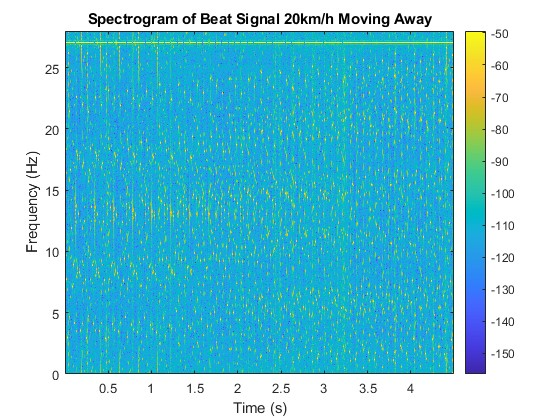
\includegraphics[scale=0.6]{pics/bab5/Velocity/2_20MA.jpg}
	\caption{Perubahan Jarak dari objek Menjauhi Radar dengan kecepatan 20 km/h pengulangan 2}
	\label{fig:pengambilan2_20MA}
\end{figure}

Pengambilan 2 20 MA

\begin{figure}
	\centering
	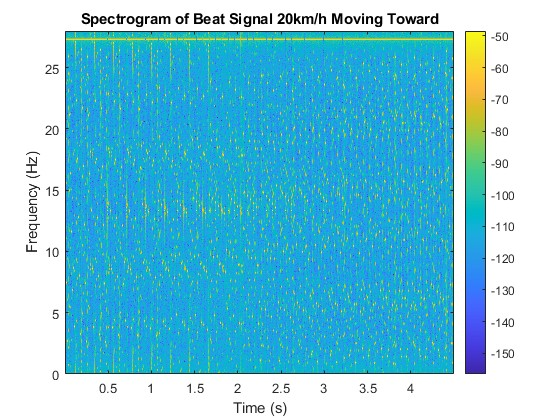
\includegraphics[scale=0.6]{pics/bab5/Velocity/2_20MT.jpg}
	\caption{Perubahan Jarak dari objek Mendekati Radar dengan kecepatan 20 km/h pengulangan 2}
	\label{fig:pengambilan2_20MT}
\end{figure}

Pengambilan 2 20 MT

\begin{figure}
	\centering
	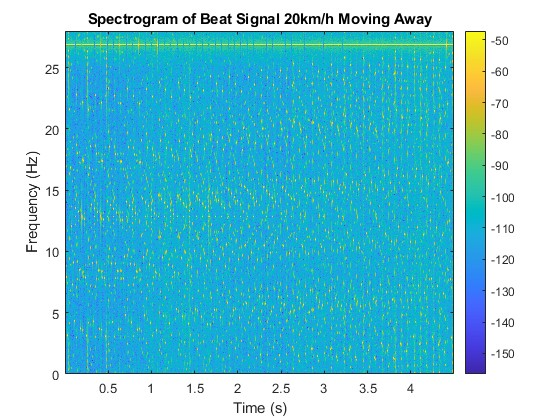
\includegraphics[scale=0.6]{pics/bab5/Velocity/3_20MA.jpg}
	\caption{Perubahan Jarak dari objek Menjauhi Radar dengan kecepatan 20 km/h pengulangan 3}
	\label{fig:pengambilan3_20MA}
\end{figure}

Pengambilan 3 20 MA

\begin{figure}
	\centering
	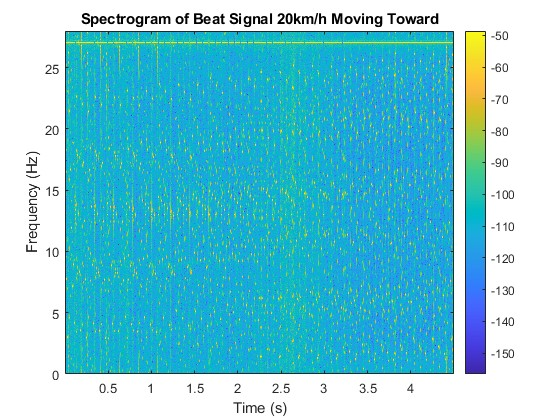
\includegraphics[scale=0.6]{pics/bab5/Velocity/3_20MT.jpg}
	\caption{Perubahan Jarak dari objek Mendekati Radar dengan kecepatan 20 km/h pengulangan 3}
	\label{fig:pengambilan3_20MT}
\end{figure}

Pengambilan 3 20 MT
%---------------------------------------------------------------
\section{Analisis Hasil}
%---------------------------------------------------------------


% \begin{center}
% 	\begin{longtable}{|c|c|c|}
% 		\caption{Hasil deteksi kecepatan menjauhi radar}
% 		\label{tab:estVelocityMoveFurther}\\
% 		\hline
% 		Kecepatan Asli & Prediksi Kecepatan & Nomor Pengujian \\
% 		\hline
% 		5 km/h & 0 & 1 \\
% 		\hline
%         5 km/h & 0 & 2\\
% 		\hline
%         5 km/h & 0 & 3\\
% 		\hline
% 		10 km/h & -9.8 km/h & 1\\
% 		\hline
%         10 km/h & 0 & 2\\
% 		\hline
%         10 km/h & 0 & 3\\
% 		\hline
% 		15 km/h & -18.03 km/h & 1\\
% 		\hline
%         15 km/h & 0 & 2\\
% 		\hline
%         15 km/h & 0 & 3\\
% 		\hline
%         20 km/h & 0 & 1\\
% 		\hline
%         20 km/h & 0 & 2\\
% 		\hline
%         20 km/h & 0 & 3\\
% 		\hline
% 	\end{longtable}
% \end{center}

% \begin{center}
% 	\begin{longtable}{|c|c|c|}
% 		\caption{Hasil deteksi kecepatan mendekati radar}
% 		\label{tab:estVelocityMoveCloser}\\
% 		\hline
% 		Kecepatan Asli & Prediksi Kecepatan & Nomor Pengujian \\
% 		\hline
% 		5 km/h & 0 & 1 \\
% 		\hline
%         5 km/h & 0 & 2\\
% 		\hline
%         5 km/h & 0 & 3\\
% 		\hline
% 		10 km/h & 10.3 km/h & 1\\
% 		\hline
%         10 km/h & 0 & 2\\
% 		\hline
%         10 km/h & 0 & 3\\
% 		\hline
% 		15 km/h & 0 & 1\\
% 		\hline
%         15 km/h & 0 & 2\\
% 		\hline
%         15 km/h & 0 & 3\\
% 		\hline
%         20 km/h & 0 & 1\\
% 		\hline
%         20 km/h & 0 & 2\\
% 		\hline
%         20 km/h & 0 & 3\\
% 		\hline
% 	\end{longtable}
% \end{center}